\documentclass[12pt, a4paper]{article}

% Standard packages for economics papers
\usepackage[utf8]{inputenc}
\usepackage[T1]{fontenc}
\usepackage{geometry}
\geometry{a4paper, margin=1in}
\usepackage{setspace}
\onehalfspacing % Common for readability; use \doublespacing if submitting for review
\usepackage{amsmath, amssymb, amsthm}
\usepackage{graphicx}
\usepackage{booktabs}  % Creates beautiful top/mid/bottom rules instead of ugly grids
\usepackage{multirow}  % Allows the p0 values to span across the T rows seamlessly
\usepackage{rotating}  % Allows for sideways tables (sidewaystable)
\usepackage{caption}
\usepackage[colorlinks=true, linkcolor=blue, citecolor=blue, urlcolor=blue]{hyperref}

% BibLaTeX setup for Zotero Better BibLaTeX
\usepackage[style=authoryear, backend=biber, natbib=true, maxcitenames=2]{biblatex}
\addbibresource{Monte Carlo Simulations.bib}

% Title and Author Information
\title{BVAR vs. Information Criteria: A Monte Carlo Simulation Study}
\author{
    Ak\i n Ayd\i n\thanks{Ludwig-Maximilian University of Munich, \href{mailto:akin.aydin@campus.lmu.de}{akin.aydin@campus.lmu.de}} \and
    Ferdinand Loser\thanks{Ludwig-Maximilian University of Munich, \href{mailto:ferdinand.loser@campus.lmu.de}{ferdinand.loser@campus.lmu.de}}
}
\date{\today}

\begin{document}

\maketitle

\begin{abstract}
\noindent
This is the abstract for your paper. Briefly state the purpose of the research, the principal results, and major conclusions. The abstract should be self-contained and citation-free. 

\vspace{1em}
\noindent\textbf{Keywords:} Monte Carlo Simulations \\
\noindent\textbf{JEL Codes:} C15, C32 % Update with relevant JEL classification codes
\end{abstract}

\newpage

\section{Introduction}
\label{sec:introduction}
Introduce the problem of lag selection and parameter proliferation in Structural VARs. Highlight the debate between hard lag selection (Information Criteria) and Bayesian methods (Shrinkage and Model Averaging).

\section{Simulation Design}
\label{sec:methodology}

This Monte Carlo simulation study follows \citet{ivanovPractitionersGuideLag2005} design with several alterations in order to make our extensions feasible and to fit the needs of our analysis. First of all, we only use one monthly DGP based on the empirical VAR study of \citet{kilianRoleInventoriesSpeculative2014}. Therefore, we do not get estimations for quarterly VAR series or VEC series and additionally do not have additional robustness by including several different series with different macroeconomic indicators and movements. The main reason for this is our tight time constraint. However, this concern is also not to be overstated as \citet{ivanovPractitionersGuideLag2005} did not find strong differences between different DGPs of the same type (monthly, quarterly, VEC). We use the dataset from \citet{kilianRoleInventoriesSpeculative2014} containing the following 4 variables: percent change in global oil production, real activity index from \citet{kilianNotAllOil2009}, the log real price of oil, and changes in OECD crude oil inventories. Just as in the original study, we first estimate a VAR with a set lag order of these 4 variables and then use the sign restrictions approach explained earlier to identify structural IRFs. Therefore, our estimation becomes much more complex and updates the findings of \citet{ivanovPractitionersGuideLag2005} to a more modern and widely used approach in the literature. All papers used for the DGP generation in \citet{ivanovPractitionersGuideLag2005} are from the 1990s and early 2000s and are based on the Cholesky decomposition approach for identification. Cholesky decomposition only gives one unique set of IRFs, whereas the sign restrictions approach principally has infinite possible sets of IRFs. 

We follow \citet{kilianRoleInventoriesSpeculative2014} in searching for a large number of admissible IRFs by randomly drawing from the space of rotation matrices. We use exactly the same sign restriction matrix, however we limit the number of periods for which dynamic sign restrictions are imposted to 3 instead of 12 and do not include additional elasticity bounds. This is a significant diversion from the original study as it makes the identification more agnostic and opens up the space of admissible IRFs. We are therefore closer to the original sign restrictions approach of \citet{uhligWhatAreEffects2005}. We understand that the additional restrictions of \citet{kilianRoleInventoriesSpeculative2014} are motivated by limiting the set to fit theory and other empirical evidence, however we have to take the less restrictive approach in order to make the estimation feasible. Especially for low lag orders and smaller samples, these restrictions have proven to be so strong that even several million draws of the rotation matrix do not give us enough admissible IRFs to make a good inference. For the simulation, this exceedingly high number of draws would need to then be repeated hundreds of times.

Out of this set we select the median target IRF as our true IRF which is defined as the IRF that has the smallest distance to the median of all admissible IRFs. The DGP follows this IRF as it is generated by a structural VAR model using the structural impact matrix $\tilde{B}$ that corresponds to the median target IRF as the parameter for the structural shocks $e_t$ which is drawn from an i.i.d. standard normal distribution. The formula for the DGP is represented by a structural VAR model using the estimated reduced form parameters $A$ (for the lag coefficients $y_{t-p}$) and $V$ (for the monthly dummy parameters $d_t$) and the structural impact matrix $\tilde{B}$ as follows:

\begin{equation}
    MSE_{relative} = \exp\left( \frac{1}{n} \sum_{i=1}^{n} \ln(r_i) \right) \text{ where } r_i=\frac{TSE_i}{TSE^{p_0}_{i}}
\end{equation}

We estimate these parameters using the original data for five different lag orders, $p_0 \in {4,6,8,10}$ and create DGPs with different sample sizes, $T \in {240, 300, 360, 480, 600}$ where $T=N+\bar{p}$. $\bar{p}$ is the set of lag orders that are considered for both the IC and the BVAR estimations, it is uniformly set to $\bar{p}=12$ to ensure that the true lag order $p_0$ is part of the set. These specifications directly follow \citet{ivanovPractitionersGuideLag2005}. We do not increase the number of lags or higher sample sizes in order to keep the comparison intact and to keep computational capacities available for the switch to sign restriction decomposition and the addition of BVAR. For sampling, we use random draws of length $p_0$ from the original dataset as initial values, then apply the parametric bootstrap using the SVAR described above and generate sequences of lengths $T$.

On each of these samples, VARs fitted by lag orders selected by both the three ICs as well as different specifications of BVAR are estimated, a fixed number of admissable IRFs found and the median target IRF determined. We estimate all BVARs using both $p=p_max=12$ and $p=p_0$ as the lag order, and can therefore compare how BVAR performs in a correctly specified model compared to a general longer lag order, as it would be applied on real data where the true lag order is unknown. The selection of the overall shrinkage parameter $lambda_1$ is the key criterion to determine how loose or how tight the prior is applied and to what extent further lag orders are shrunk towards 0. We apply $\lambda_1 \in \{0.05, 0.2, 0.35, 0.5, 0.65, 0.8, 0.95\}$ to determine how optimal shrinkage depends on sample size $T$ and true lag order $p_0$. Additionally, we use the marginal data density (MDD) method to determine a $lambda_1$ optimized on Out-of-Sample MSE for which we also provide the same set of admissable $\lambda_1$-values. The limitation of the value-field is established for computational reasons, it captures a good range of typically used $lambda_1$-values, both tighter and looser specifications. 

Finally, the squared error matrix of the selected median target IRF to the true DGP IRF is calculated, collapsed into a scalar total squared error by summation. Then we estimate the ratio of this squared error of a specific estimation approach to the model fitted by the true lag order $p_0$. Therefore, the deviations of the true IRF are directly put into relation to how well a correctly specified model compares for the given sample. Finally, we estimate the MSE by calculating the geometric mean of these individual ratios. The geometric mean is preferred over the arithmetic mean as the ratios are bounded for outperformance at 0 and unbounded for performing worse than the correctly specified model. Outliers on the right side are hence overweighted in the arithmetic mean. The relative MSE for one method for one true lag order $p_0$ and one sample size $T$ is given by the following formula:

\begin{equation}
    MSE_{relative} = \exp\left( \frac{1}{n} \sum_{i=1}^{n} \ln(r_i) \right) \text{ where } r_i=\frac{TSE_i}{TSE_{p_0}}
\end{equation}

While, for a single estimation it is possible to estimate millions of admissable IRFs, the Monte Carlo simulation approach doesn't allow for such a large number of draws. In establishing the median target IRF specific to the DGP, we set the number of discovered admissible IRFs to 1 million so as to have a very accurate median target IRF for the specific dataset. In the Monte Carlo Simulation, we reduce this number drastically to 100 as it has proven to be the absolute limit that still allows us to have an acceptable number of Monte Carlo iterations, 1000, for our set of different methods. Even with computational optimization by parallel processing, more draws are not applicable under our hardware constraints. For each individual iteration, the median target IRF is therefore less accurately determined. However, because we use relative MSEs as our performance measure and repeat the process 1000 times, this should not impact the interpretability of our results. 

\section{Results}
\label{sec:results}

% Placing the MDD Surface here visually justifies your optimization approach.
\begin{figure}[htbp]
    \centering
    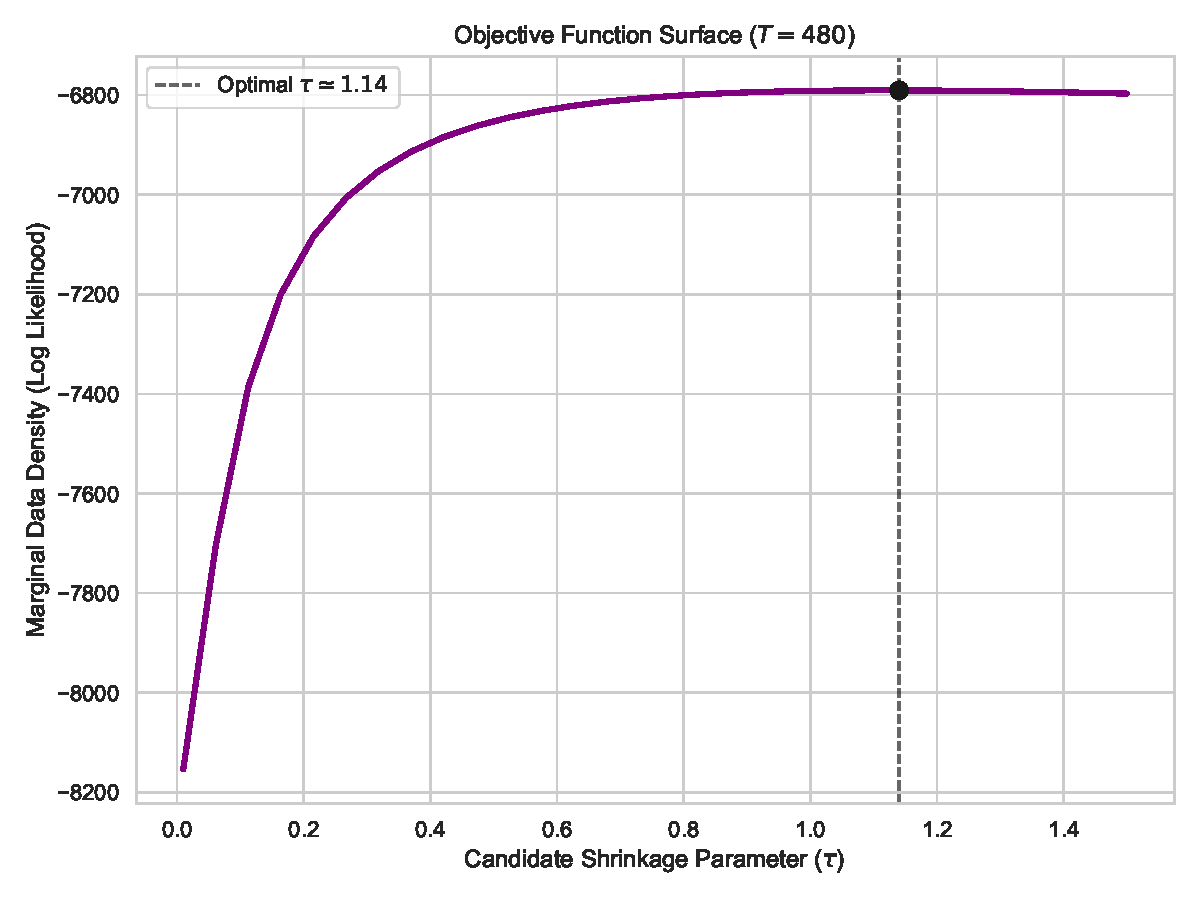
\includegraphics[width=0.85\textwidth]{Figures/Fig3_MDD_Surface.pdf}
    \caption{Objective Function Surface for Marginal Data Density Optimization. The peak represents the optimal balance between model fit and parameter penalty.}
    \label{fig:mdd_surface}
\end{figure}

Present the results of the Monte Carlo simulations, broken down by the specific strategies employed to handle model uncertainty.

\subsection{Behavior of Standard Information Criteria}
As established theoretically as well as in the foundational Monte Carlo simulation study on information criterias, \citet{lutkepohlComparisonCriteriaEstimating1985}, AIC tends to select higher lag orders than HQC and BIC, and BIC typically has the strongest reduction in included lags. Our results confirm this as seen in \ref{tab:ic_lag_orders}.

\begin{table}[htbp]
\centering
\caption{Average Evaluated Lag Order ($\hat{p}$) selected by Information Criteria.}
\label{tab:ic_lag_orders}
\begin{tabular}{llccc}
\toprule
 & Estimator & AIC & BIC & HQC \\
$p_0$ & $T$ &  &  &  \\
\midrule
\multirow[t]{2}{*}{4} & 240 & 2.99 & 1.95 & 2.06 \\
 & 600 & 3.80 & 2.02 & 2.66 \\
\multirow[t]{2}{*}{10} & 240 & 6.54 & 1.96 & 2.07 \\
 & 600 & 9.16 & 2.02 & 4.03 \\
\bottomrule
\end{tabular}
\end{table}


\subsection{The Shrinkage Strategy: Priors vs. Data}
This section compares hard lag selection against dynamic BVARs. We analyze both the bias-variance tradeoff and how the optimal prior relaxes asymptotically as sample sizes increase.

\begin{sidewaystable}[htbp]
\centering
\caption{Relative Mean Squared Error: Hard Selection vs.~Bayesian Shrinkage.}
\label{tab:shrinkage_mse}
\begin{tabular}{llccccccccccccc}
\toprule
 &  & AIC & BIC & HQC & \begin{tabular}{@{}c@{}}BVAR \\ ($\lambda_1=0.05$)\end{tabular} & \begin{tabular}{@{}c@{}}BVAR \\ ($\lambda_1=0.20$)\end{tabular} & \begin{tabular}{@{}c@{}}BVAR \\ ($\lambda_1=0.35$)\end{tabular} & \begin{tabular}{@{}c@{}}BVAR \\ ($\lambda_1=0.50$)\end{tabular} & \begin{tabular}{@{}c@{}}BVAR \\ ($\lambda_1=0.65$)\end{tabular} & \begin{tabular}{@{}c@{}}BVAR \\ ($\lambda_1=0.80$)\end{tabular} & \begin{tabular}{@{}c@{}}BVAR \\ ($\lambda_1=0.95$)\end{tabular} & \begin{tabular}{@{}c@{}}BVAR RW \\ ($\lambda_1=0.20$)\end{tabular} & \begin{tabular}{@{}c@{}}BVAR RW \\ ($\lambda_1=0.50$)\end{tabular} & \begin{tabular}{@{}c@{}}BVAR \\ (MDD $\lambda_1$)\end{tabular} \\
$T$ & $p_0$ &  &  &  &  &  &  &  &  &  &  &  &  &  \\
\midrule
\multirow[t]{4}{*}{240} & 4 & 0.818 & \bfseries 0.254 & 0.596 & 1.333 & 0.484 & 1.662 & 0.599 & 0.555 & 1.560 & 0.741 & 0.610 & 1.682 & 0.484 \\
 & 6 & 1.511 & 0.899 & 0.899 & 2.649 & 1.568 & 0.965 & 1.212 & 1.071 & 0.997 & 1.094 & \bfseries 0.719 & 0.936 & 1.568 \\
 & 8 & 0.634 & 1.068 & 0.943 & \bfseries 0.267 & 0.924 & 0.738 & 1.354 & 0.712 & 0.972 & 0.778 & 1.294 & 0.909 & 0.924 \\
 & 10 & 0.369 & \bfseries 0.358 & \bfseries 0.358 & 2.264 & 1.708 & 0.614 & 1.667 & 1.652 & 0.799 & 0.688 & 2.417 & 1.426 & 1.708 \\
\multirow[t]{4}{*}{300} & 4 & 0.709 & 0.639 & 1.280 & 1.732 & 1.074 & 0.426 & \bfseries 0.315 & 0.676 & 0.863 & 0.733 & 0.353 & 0.991 & 1.074 \\
 & 6 & 0.340 & 1.012 & 1.012 & 1.043 & 1.051 & 0.915 & 0.629 & 0.933 & 1.853 & 0.664 & 1.216 & \bfseries 0.324 & 1.051 \\
 & 8 & \bfseries 0.695 & 4.300 & 4.300 & 8.912 & 1.390 & 2.032 & 2.970 & 1.751 & 1.432 & 1.546 & 3.712 & 7.187 & 1.390 \\
 & 10 & 0.331 & 0.689 & 0.689 & 0.621 & 0.508 & 0.442 & 1.164 & 0.301 & 0.565 & 0.427 & \bfseries 0.212 & 0.460 & 0.508 \\
\multirow[t]{4}{*}{360} & 4 & \bfseries 1.000 & 4.401 & 4.401 & 1.552 & 3.960 & 2.886 & 2.818 & 2.133 & 4.419 & 4.102 & 1.065 & 1.822 & 3.960 \\
 & 6 & 0.742 & 1.641 & 1.641 & 2.622 & \bfseries 0.259 & 3.590 & 0.630 & 1.446 & 1.667 & 2.220 & 1.327 & 0.746 & \bfseries 0.259 \\
 & 8 & 1.000 & 0.917 & 1.242 & 0.848 & 0.590 & 0.977 & 1.618 & \bfseries 0.225 & 1.112 & 1.021 & 0.590 & 1.682 & 0.590 \\
 & 10 & 2.034 & \bfseries 0.720 & \bfseries 0.720 & 0.854 & 1.905 & 1.760 & 0.896 & 1.022 & 1.315 & 1.763 & 1.349 & 2.209 & 1.905 \\
\multirow[t]{4}{*}{480} & 4 & 1.000 & 0.256 & 1.000 & 1.135 & 0.338 & 0.892 & \bfseries 0.164 & 0.836 & 0.908 & 1.142 & 0.803 & 0.793 & 0.338 \\
 & 6 & 0.889 & 1.978 & 1.758 & 4.208 & 4.130 & 3.993 & 1.523 & \bfseries 0.847 & 4.076 & 2.191 & 4.107 & 2.194 & 4.130 \\
 & 8 & 1.000 & 2.663 & 2.663 & 1.610 & 2.021 & 1.861 & 1.351 & 1.327 & 1.120 & 2.140 & \bfseries 0.591 & 1.679 & 2.021 \\
 & 10 & 0.260 & 1.050 & 1.050 & 0.447 & 0.500 & 0.553 & 0.218 & 0.864 & 0.354 & \bfseries 0.162 & 0.324 & 0.426 & 0.500 \\
\multirow[t]{4}{*}{600} & 4 & 0.915 & 0.629 & 0.915 & 1.289 & 0.582 & 0.551 & 0.443 & 0.560 & 0.510 & \bfseries 0.277 & 0.325 & 0.472 & 0.582 \\
 & 6 & 1.000 & 1.916 & 1.446 & 0.939 & 1.335 & 2.567 & 1.364 & 1.781 & 1.728 & \bfseries 0.615 & 1.731 & 2.427 & 1.335 \\
 & 8 & 1.000 & 1.568 & 0.799 & 6.511 & 4.181 & 1.105 & 4.780 & \bfseries 0.643 & 3.925 & 5.541 & 6.511 & 1.557 & 1.105 \\
 & 10 & 2.294 & 0.899 & 1.437 & 1.134 & 1.539 & 0.827 & 2.074 & 2.509 & 1.117 & 1.313 & \bfseries 0.594 & 1.796 & 0.827 \\
\bottomrule
\end{tabular}
\end{sidewaystable}


\ref{fig:tradeoff} illustrates how BVAR performs in comparison to BIC for $T=240$ and $T=600$ at $p_0=4$ at the different values of $\lambda_1$.

\begin{figure}[htbp]
    \centering
    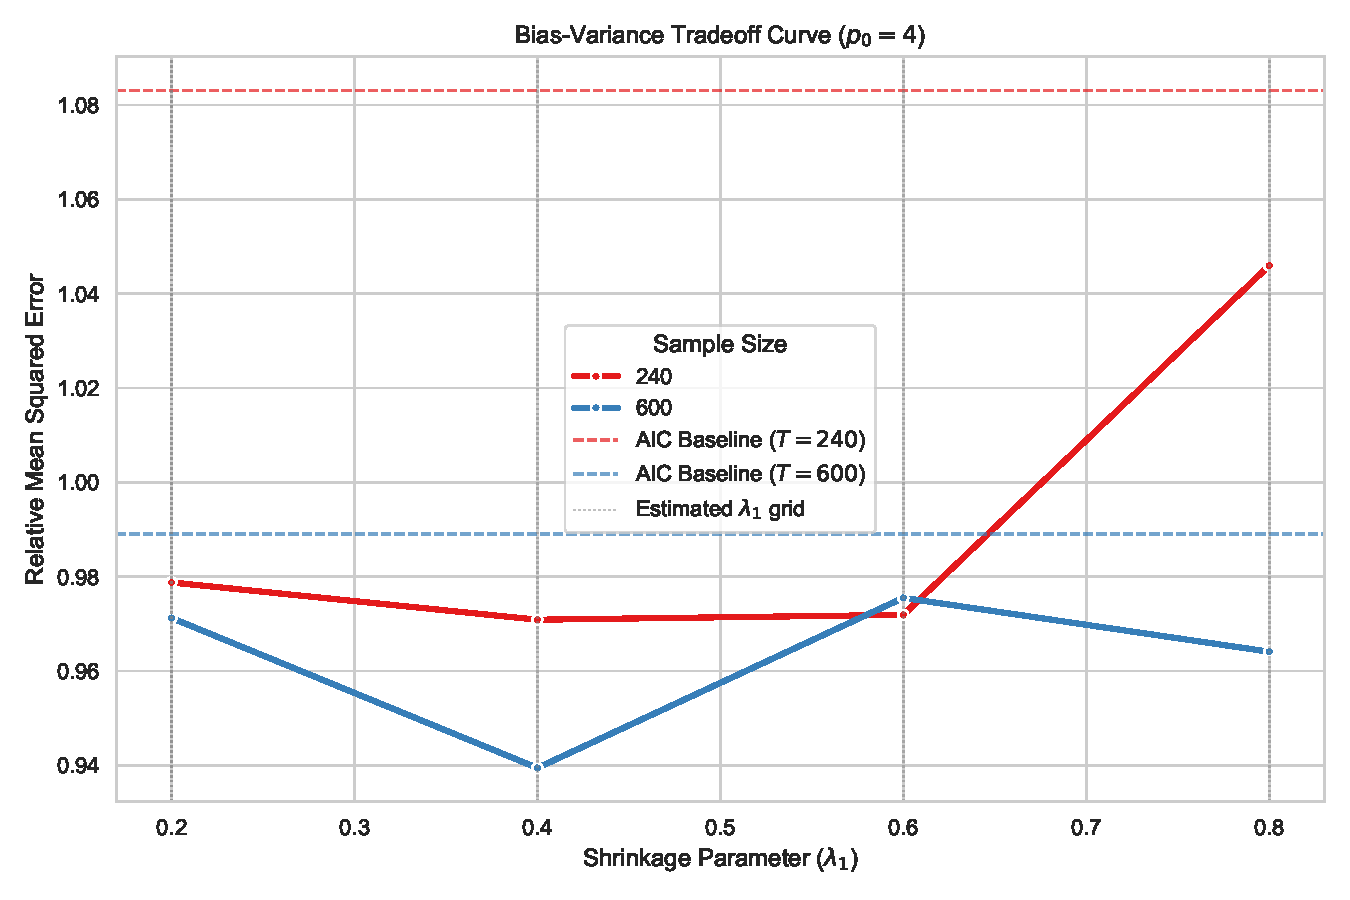
\includegraphics[width=0.85\textwidth]{Figures/Fig1_Tradeoff_Curve.pdf}
    \caption{Comparison of Bias-Variance Tradeoff: BVAR vs. Hard Selection. The curve illustrates how the optimal $\tau$ balances bias and variance, achieving superior MSE performance compared to fixed lag selection.}
    \label{fig:tradeoff}
\end{figure}

Finally, we can compare how BVAR using the true lag order $p_0$ performs in comparison to BVAR with $p_{max}$. We include this to find out whether the shrinkage of BVAR is strong enough to reduce an overfitted model to achieve good results or whether a more accurate lag order selection is highly beneficial to the BVAR approach. Additionally, we can reveal whether optimal $\lambda_1$-values change when the pre-determined lag order changes. \ref{tab:p0_vs_pmax} shows the relative MSE of the BVAR fitted with $p_0$ with the BVAR fitted with $p_{max}$. Cases where $p_0$ outperforms our baseline, i.e. $MSE<1$ are shown in bold. 

\begin{table}[htbp]
\centering
\caption{Ratio of Relative MSE: Estimating with True Lag Order ($p_0$) vs. Maximum Lag Order ($p_{\max}$). Values $< 1.0$ indicate $p_0$ outperforms $p_{\max}$.}
\label{tab:p0_vs_pmax}
\begin{tabular}{llcccccccc}
\toprule
 &  & \begin{tabular}{@{}c@{}}$\lambda_1$ \\ 0.05\end{tabular} & \begin{tabular}{@{}c@{}}$\lambda_1$ \\ 0.20\end{tabular} & \begin{tabular}{@{}c@{}}$\lambda_1$ \\ 0.35\end{tabular} & \begin{tabular}{@{}c@{}}$\lambda_1$ \\ 0.50\end{tabular} & \begin{tabular}{@{}c@{}}$\lambda_1$ \\ 0.65\end{tabular} & \begin{tabular}{@{}c@{}}$\lambda_1$ \\ 0.80\end{tabular} & \begin{tabular}{@{}c@{}}$\lambda_1$ \\ 0.95\end{tabular} & \begin{tabular}{@{}c@{}}MDD \\ $\lambda_1$\end{tabular} \\
$T$ & $p_0$ &  &  &  &  &  &  &  &  \\
\midrule
\multirow[t]{4}{*}{240} & 4 & \bfseries 0.126 & \bfseries 0.583 & 1.508 & 1.592 & 1.961 & \bfseries 0.749 & 1.035 & \bfseries 0.583 \\
 & 6 & \bfseries 0.951 & 1.108 & \bfseries 0.967 & \bfseries 0.222 & \bfseries 0.609 & \bfseries 0.643 & \bfseries 0.420 & 1.108 \\
 & 8 & 2.460 & 2.385 & 3.265 & 3.089 & 1.030 & \bfseries 0.802 & 1.676 & 2.385 \\
 & 10 & \bfseries 0.521 & \bfseries 0.742 & \bfseries 0.976 & \bfseries 0.819 & 3.949 & 1.778 & \bfseries 0.829 & \bfseries 0.742 \\
\multirow[t]{4}{*}{300} & 4 & 1.382 & 6.007 & \bfseries 0.555 & \bfseries 0.863 & 1.605 & 1.860 & 2.673 & 6.007 \\
 & 6 & 3.113 & 1.072 & 2.131 & \bfseries 0.977 & 1.369 & \bfseries 0.595 & 1.077 & 1.072 \\
 & 8 & 6.684 & \bfseries 0.191 & \bfseries 0.519 & \bfseries 0.514 & \bfseries 0.228 & \bfseries 0.194 & \bfseries 0.576 & \bfseries 0.191 \\
 & 10 & 1.071 & \bfseries 0.919 & \bfseries 0.440 & 1.749 & \bfseries 0.642 & \bfseries 0.520 & \bfseries 0.668 & \bfseries 0.472 \\
\multirow[t]{4}{*}{360} & 4 & \bfseries 0.674 & 2.783 & \bfseries 0.086 & \bfseries 0.061 & \bfseries 0.641 & 1.471 & \bfseries 0.318 & 2.783 \\
 & 6 & 1.560 & 5.719 & 1.035 & 2.212 & \bfseries 0.694 & 1.090 & \bfseries 0.199 & 5.719 \\
 & 8 & \bfseries 0.380 & \bfseries 0.100 & 2.063 & \bfseries 0.449 & \bfseries 0.531 & \bfseries 0.453 & \bfseries 0.139 & \bfseries 0.100 \\
 & 10 & 2.072 & 2.409 & 5.660 & 1.497 & \bfseries 0.317 & \bfseries 0.812 & \bfseries 0.816 & 2.409 \\
\multirow[t]{4}{*}{480} & 4 & 3.874 & \bfseries 0.976 & 1.812 & \bfseries 0.487 & 1.569 & 2.270 & \bfseries 0.868 & \bfseries 0.778 \\
 & 6 & \bfseries 0.152 & 1.073 & 2.227 & \bfseries 0.736 & 1.306 & 1.038 & 2.858 & 2.466 \\
 & 8 & 2.138 & \bfseries 0.698 & \bfseries 0.972 & \bfseries 0.435 & \bfseries 0.573 & \bfseries 0.549 & 1.032 & \bfseries 0.571 \\
 & 10 & \bfseries 0.334 & 2.382 & 1.723 & 1.308 & 1.285 & 1.214 & \bfseries 0.838 & 2.866 \\
\multirow[t]{4}{*}{600} & 4 & 1.007 & \bfseries 0.631 & \bfseries 0.310 & \bfseries 0.537 & 1.138 & \bfseries 0.673 & 1.032 & \bfseries 0.179 \\
 & 6 & 1.062 & \bfseries 0.843 & \bfseries 0.843 & \bfseries 0.928 & \bfseries 0.896 & 1.518 & \bfseries 0.507 & \bfseries 0.843 \\
 & 8 & \bfseries 0.494 & 1.419 & 1.198 & \bfseries 0.640 & \bfseries 0.935 & \bfseries 0.624 & 2.137 & 1.075 \\
 & 10 & 1.384 & \bfseries 0.524 & \bfseries 0.365 & \bfseries 0.332 & \bfseries 0.087 & 1.515 & 1.166 & \bfseries 0.365 \\
\bottomrule
\end{tabular}
\end{table}


\begin{figure}[htbp]
    \centering
    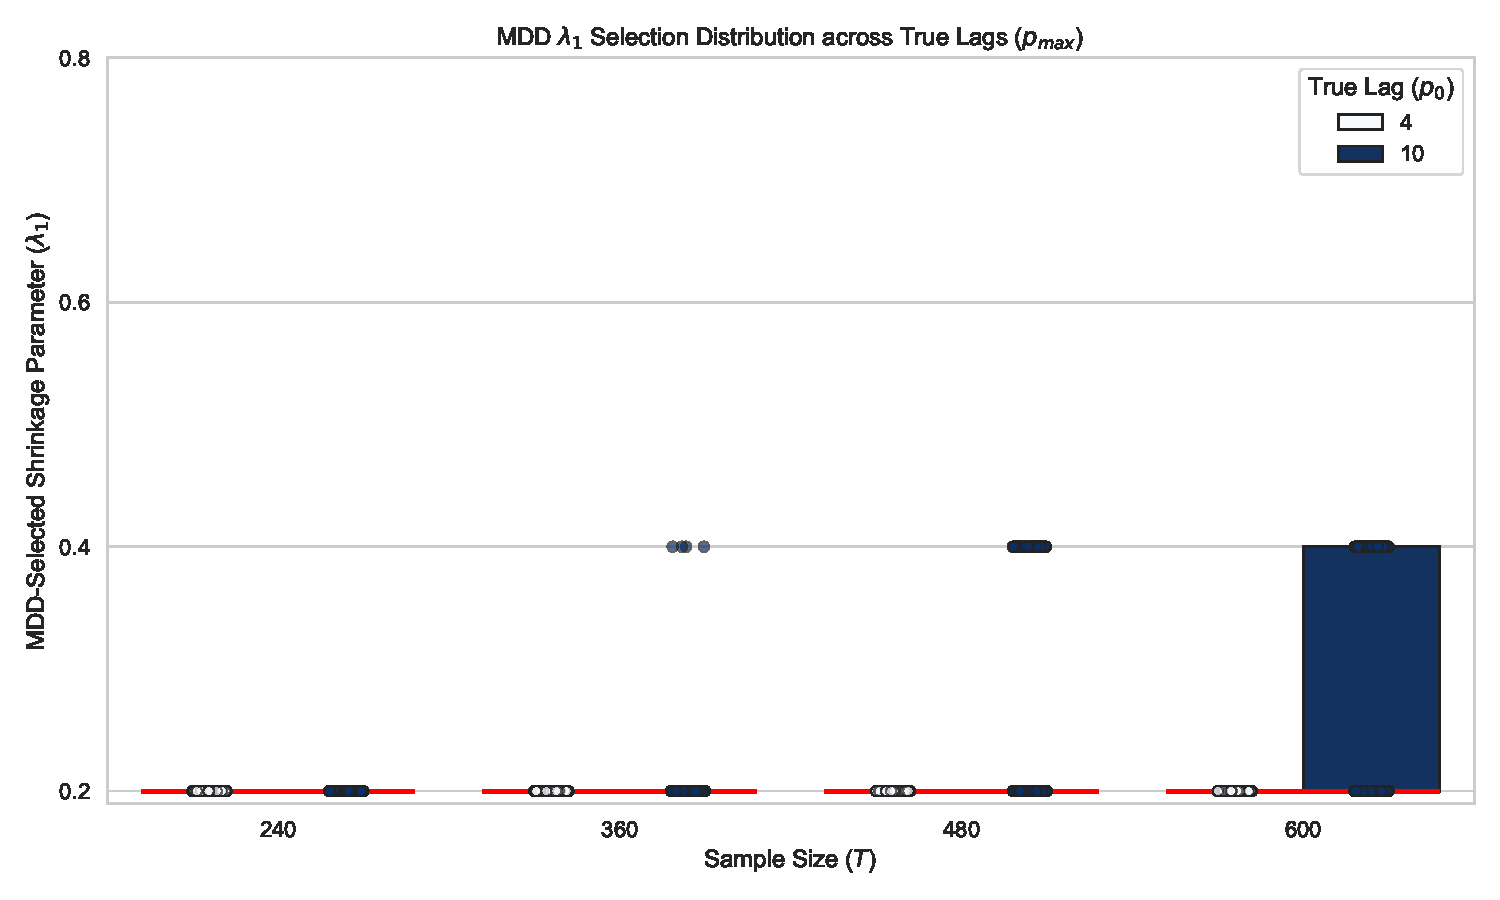
\includegraphics[width=0.85\textwidth]{Figures/Fig2_Asymptotic_Relaxation.pdf}
    \caption{The MDD selected priors for different sample sizes for $p=p_{max}=12$, $p=p_{0}=4$.}
    \label{fig:asymptotic_relaxation}
\end{figure}

\begin{figure}[htbp]
    \centering
    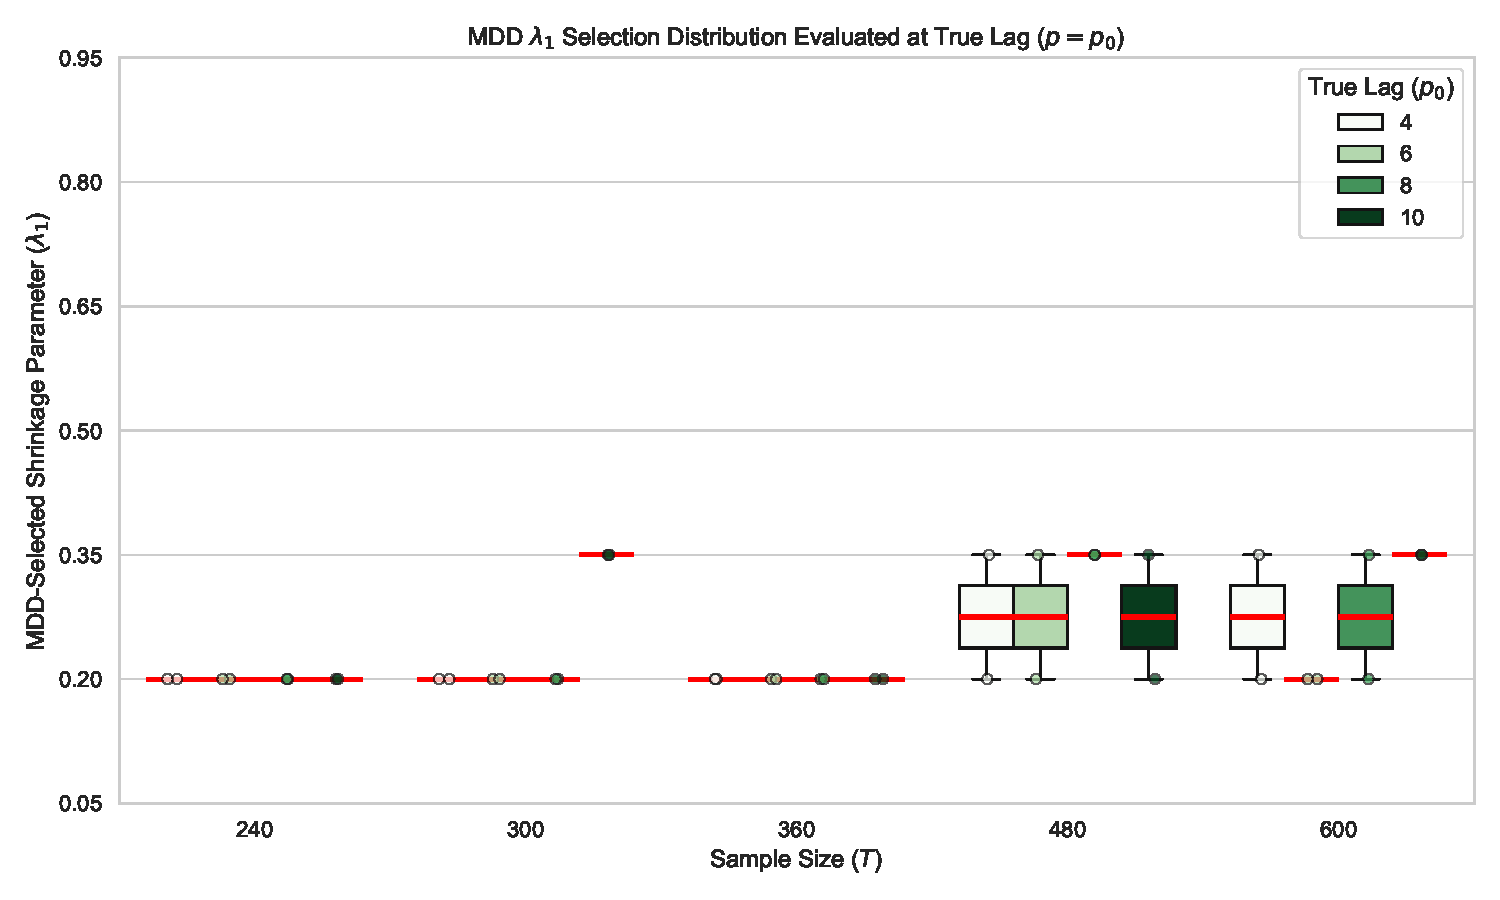
\includegraphics[width=0.85\textwidth]{Figures/Fig2b_Asymptotic_Relaxation_p0.pdf}
    \caption{The MDD selected priors for different sample sizes for $p=p_{0}=12$.}
    \label{fig:asymptotic_relaxation_p0}
\end{figure}

\clearpage
\section{Conclusion}
\label{sec:conclusion}

Summarize the main findings, specifically highlighting how optimal $\tau$ selection and true BMA systematically outperform standard econometric heuristics in finite samples.

\newpage
% Print the bibliography

\section*{References}
\printbibliography

\section*{Declaration of AI Usage}

During the preparation of this seminar paper, I, [NAME], used Claude, Gemini, and ChatGPT for help with coding, research, and adapting writing to academic standards. I have reviewed and edited the content as needed and take full responsibility for the content.

[NAME]

\end{document}